\documentclass[11pt,a4paper]{article}
\usepackage[utf8]{inputenc}
\usepackage[T1]{fontenc}
\usepackage[margin=2.05cm]{geometry}
\usepackage{microtype,booktabs,tabularx,array,amsmath,amssymb,mathtools,graphicx,float,caption,subcaption,hyperref,siunitx,bm}
\graphicspath{{../figures/main/}{../figures/si/}}
\hypersetup{colorlinks=true,linkcolor=blue,citecolor=teal,urlcolor=teal}

\title{How CO$_2$/N$_2$ Selectivity Emerges in Metal--Organic Frameworks:\\Repulsive Baselines, Attractive Reversal, and Electrostatic Recognition}
\author{Author list to be finalized}
\date{}

\begin{document}
\maketitle

\begin{abstract}
High-throughput screening ranks metal--organic frameworks (MOFs) by adsorption performance, but a final selectivity does not reveal which intermolecular interactions produced it. We construct a nested reference-potential decomposition of Henry-regime CO$_2$/N$_2$ selectivity across 238 MOFs, separating a repulsive Weeks--Chandler--Andersen (WCA) reference from the increments obtained by restoring Lennard--Jones attraction and then electrostatics. Repulsive accessibility alone favored N$_2$ in every framework (median $S_{\rm WCA}=0.816$). Restoring attraction reversed this preference throughout the panel, with a median $\Delta\ln S_{\rm attr}=2.537$ (12.65-fold), whereas electrostatics supplied a further positive but strongly framework-dependent increment (median $\Delta\ln S_{\rm elec}=0.309$, 1.36-fold). The attractive and electrostatic increments were only weakly associated ($\rho=-0.089$). Conventional pore geometry predicted the WCA and attractive coordinates strongly ($R^2=0.835$ and 0.874) and also predicted the final selectivity ($R^2=0.845$), yet provided essentially no reduction in mean absolute error for the electrostatic increment relative to a median predictor (0.146 versus 0.147). A geometry-matched pair makes this representation boundary explicit: M029 and M085 are mutual nearest neighbors in the geometry space but have electrostatic increments of 0.141 and 2.001. Global Henry coefficients and probability-supported spatial fields show that this contrast is overwhelmingly CO$_2$-driven and is accompanied by a markedly different local electrostatic response. The results show that accurate endpoint prediction can conceal missing mechanistic information and provide a controlled route for separating accessibility, attraction, and electrostatic recognition in MOF screening.
\end{abstract}

\section{Introduction}

Metal--organic frameworks (MOFs) provide a large design space for adsorption-based separations, and high-throughput molecular simulation has become a standard way to screen that space \cite{haldoupis2012charges,burner2023arcmof}. For post-combustion CO$_2$/N$_2$ separation, screening studies commonly reduce each framework to quantities such as uptake, Henry coefficient, working capacity, or selectivity. These endpoints are useful for ranking materials, but they do not state which intermolecular interactions made a framework selective.

The importance of electrostatics in CO$_2$/N$_2$ adsorption is already well established. Haldoupis, Nair, and Sholl showed that reliable charge assignment is central to large-scale screening of quadrupolar CO$_2$ and N$_2$ \cite{haldoupis2012charges}. In a later screening of 3,806 MOFs, Daglar and Keskin explicitly repeated simulations with framework electrostatics removed and found substantial changes in CO$_2$/N$_2$ adsorption performance and in the identity of top candidates \cite{daglar2018screening}. Such comparisons establish that electrostatics matters, but a full-versus-uncharged comparison still combines steric exclusion and dispersive attraction in the same non-electrostatic reference.

A parallel literature asks how much adsorption performance can be inferred from structure alone. Geometry-based descriptors can provide effective low-cost filters for CO$_2$ and N$_2$ adsorption \cite{fernandez2016geometry}, whereas large-scale machine-learning studies have shown that chemistry-aware descriptors can substantially improve low-pressure CO$_2$ working-capacity and CO$_2$/N$_2$ selectivity prediction beyond geometry-only models \cite{burner2020deeplearning}. These results establish a representation hierarchy for endpoint prediction. They do not, however, identify which physical contribution is captured or missed by a representation.

Here we connect these two questions. We construct a nested sequence of reference potentials that separates repulsive accessibility, Lennard--Jones attraction, and electrostatic recognition for the same framework population. The WCA construction provides the repulsive Lennard--Jones reference \cite{weeks1971wca}; related WCA splitting has previously been used to isolate repulsive contributions in MOF adsorption models \cite{campbell2018polar}. Restoring the full Lennard--Jones potential then introduces attraction, and restoring framework--guest electrostatics gives the complete model:
\begin{equation}
\ln S_{\rm full}
=
\ln S_{\rm WCA}
+
\Delta\ln S_{\rm attr}
+
\Delta\ln S_{\rm elec},
\end{equation}
with
$\Delta\ln S_{\rm attr}=\ln S_{\rm LJ}-\ln S_{\rm WCA}$
and
$\Delta\ln S_{\rm elec}=\ln S_{\rm full}-\ln S_{\rm LJ}$.
These are controlled finite differences between reference potentials, not uniquely separable experimental free-energy components.

Across 238 MOFs, we ask which interaction stage first creates CO$_2$ preference, whether attractive and electrostatic enhancements track one another, and which of these coordinates is encoded by conventional pore geometry. We then use a geometry-matched pair and local insertion fields to test whether a large electrostatic increment corresponds to a distinct spatial response. The resulting picture is sequential rather than symmetric: repulsion sets an N$_2$-favoring baseline, attraction creates CO$_2$ selectivity throughout this panel, and electrostatics provides an additional framework-specific recognition channel that conventional pore geometry does not adequately resolve.

\section{Results}

\subsection{Repulsion sets the baseline and attraction creates CO$_2$ preference}

The common analysis set contains 238 MOFs evaluated in WCA, LJ-only, and full interaction states. The nested identity closes numerically to a maximum residual of $8.88\times10^{-16}$.

Under the WCA reference, all 238 frameworks are N$_2$-favoring. The median $\ln S_{\rm WCA}$ is $-0.204$, corresponding to a median $S_{\rm WCA}=0.816$. Repulsive accessibility therefore does not constitute a successful CO$_2$-selectivity route in this population.

Restoring attractive Lennard--Jones interactions changes the result qualitatively. $\Delta\ln S_{\rm attr}$ is positive for every framework, with a median of 2.537, corresponding to a 12.65-fold multiplicative contribution. The LJ-only selectivity is CO$_2$-favoring throughout the panel. Attraction is therefore the interaction stage that reverses the repulsive N$_2$ preference and establishes CO$_2$ selectivity under these models.

\begin{figure}[H]
\centering
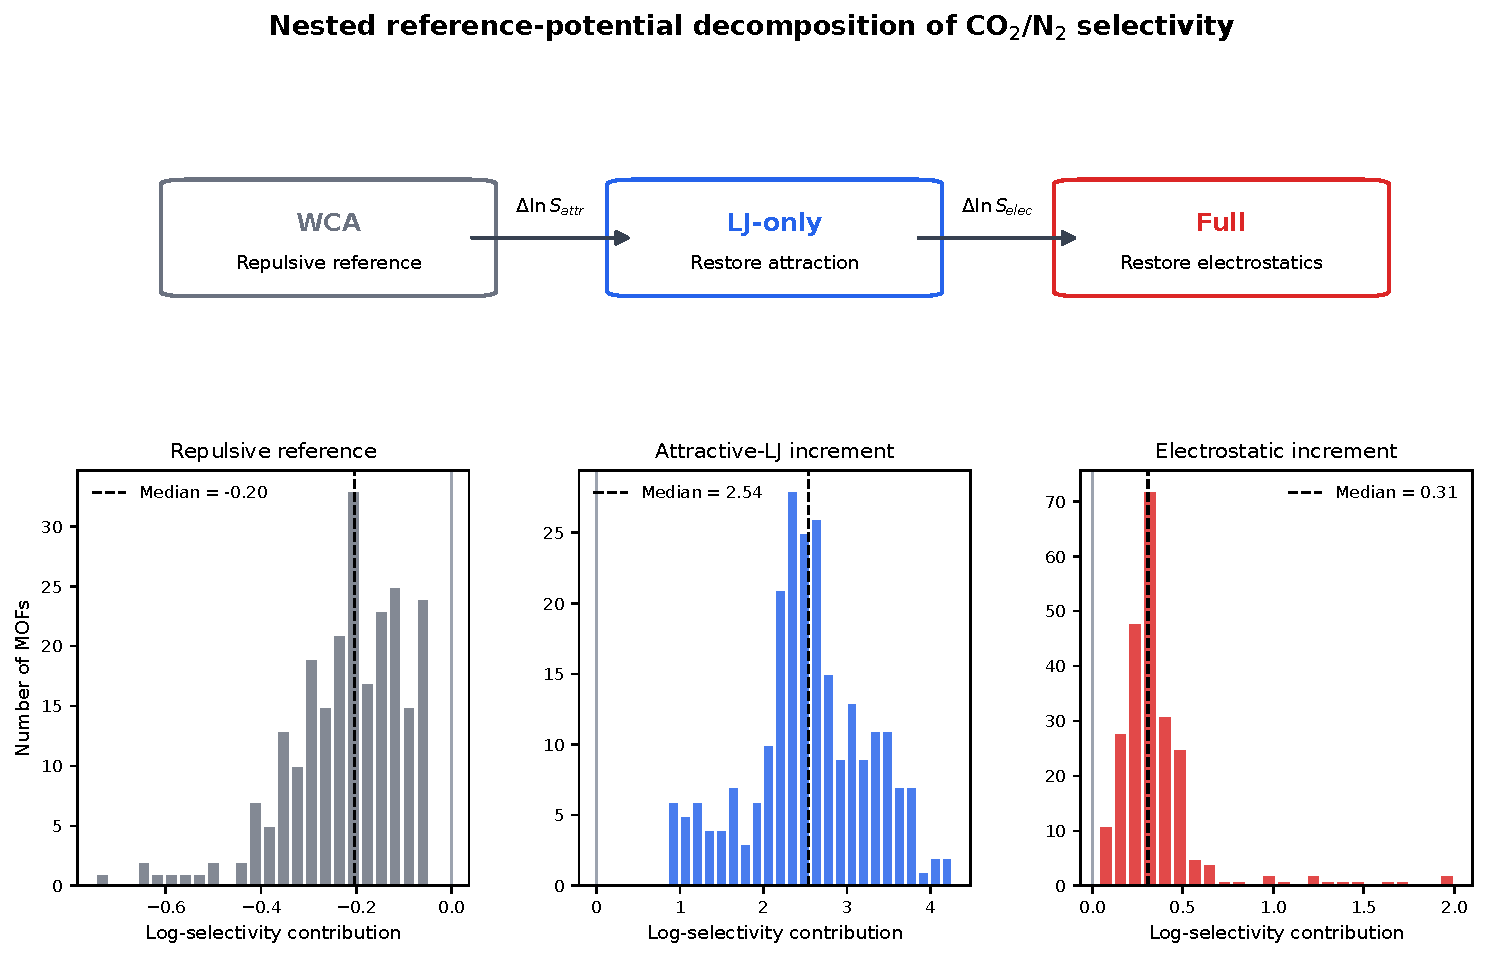
\includegraphics[width=\linewidth]{fig1_decomposition.pdf}
\caption{\textbf{Nested reference-potential decomposition of CO$_2$/N$_2$ selectivity.} The WCA state retains repulsive accessibility, the LJ-only state restores attractive Lennard--Jones interactions, and the full state additionally restores electrostatics. The population distributions reveal an N$_2$-favoring repulsive baseline, a positive attractive increment throughout the panel, and a positive but more heterogeneous electrostatic increment.}
\label{fig:decomp}
\end{figure}

\subsection{Attraction and electrostatics are weakly associated across the population}

Restoring electrostatics provides a further positive enhancement in every framework. The median $\Delta\ln S_{\rm elec}$ is 0.309, equivalent to a 1.36-fold multiplicative contribution, while the largest increments approach 2 log units.

The attractive and electrostatic increments are only weakly associated across the population (Spearman $\rho=-0.089$; Figure~\ref{fig:map}). A framework's gain from attractive confinement therefore provides little information about the additional gain it receives from electrostatic interactions. This does not imply statistical independence; it shows that the two finite-difference coordinates encode substantially different framework-to-framework variation.

\begin{figure}[H]
\centering
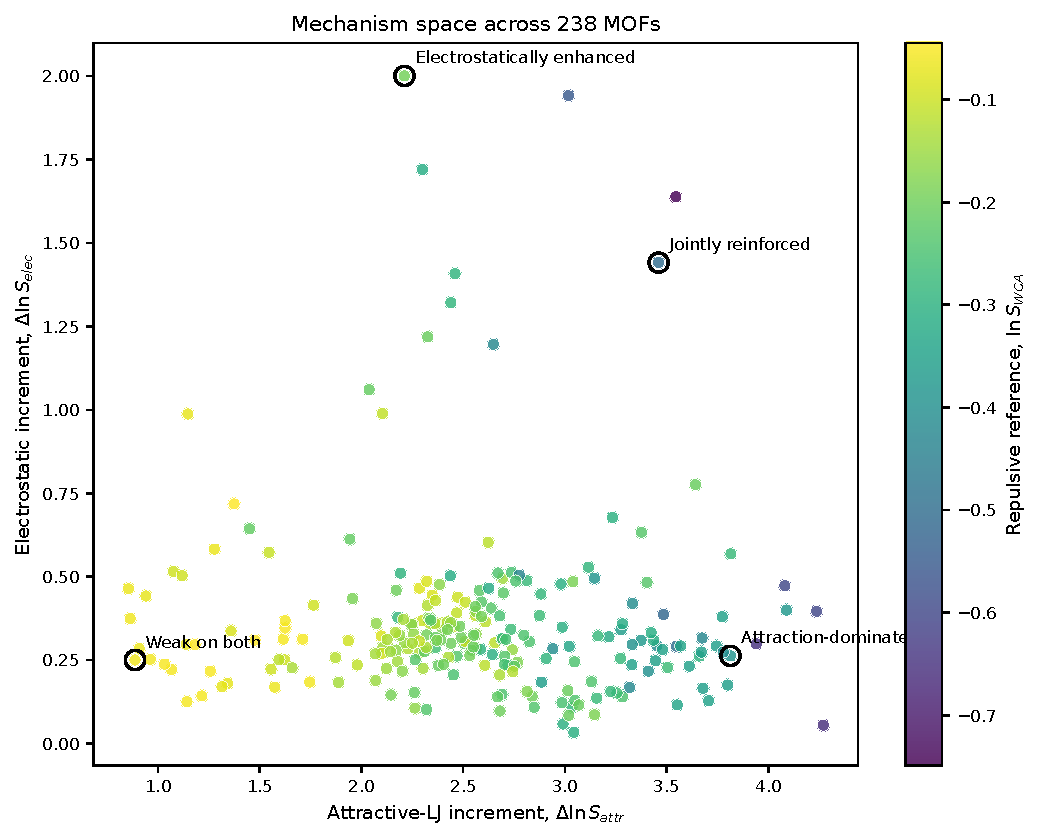
\includegraphics[width=.78\linewidth]{fig2_mechanism_map.pdf}
\caption{\textbf{Attractive and electrostatic enhancements are weakly associated across 238 MOFs.} Each point is one framework. The frozen attraction- and electrostatic-matched pairs are highlighted only as case studies; no categorical mechanism boundaries are imposed on the population.}
\label{fig:map}
\end{figure}

\subsection{Geometry predicts the endpoint while missing the electrostatic increment}

We next ask how much information about each mechanistic coordinate is already available from conventional pre-simulation pore geometry. ExtraTrees models using 14 geometry descriptors give five-fold cross-validated $R^2=0.835$ for $\ln S_{\rm WCA}$ and $R^2=0.874$ for $\Delta\ln S_{\rm attr}$. Their mean absolute errors are 0.033 and 0.177, compared with median-predictor baselines of 0.093 and 0.549.

The electrostatic increment behaves differently. Geometry gives $R^2=0.188$, but its MAE of 0.146 is essentially identical to the baseline MAE of 0.147. Thus the descriptors retain some population-level association with $\Delta\ln S_{\rm elec}$, yet provide almost no practical gain in absolute prediction error. In contrast, the same geometry set predicts the final $\ln S_{\rm full}$ well ($R^2=0.845$; MAE 0.189 versus a 0.501 baseline). Accurate prediction of the endpoint therefore does not imply that the representation resolves every interaction contribution used to construct that endpoint.

\begin{figure}[H]
\centering
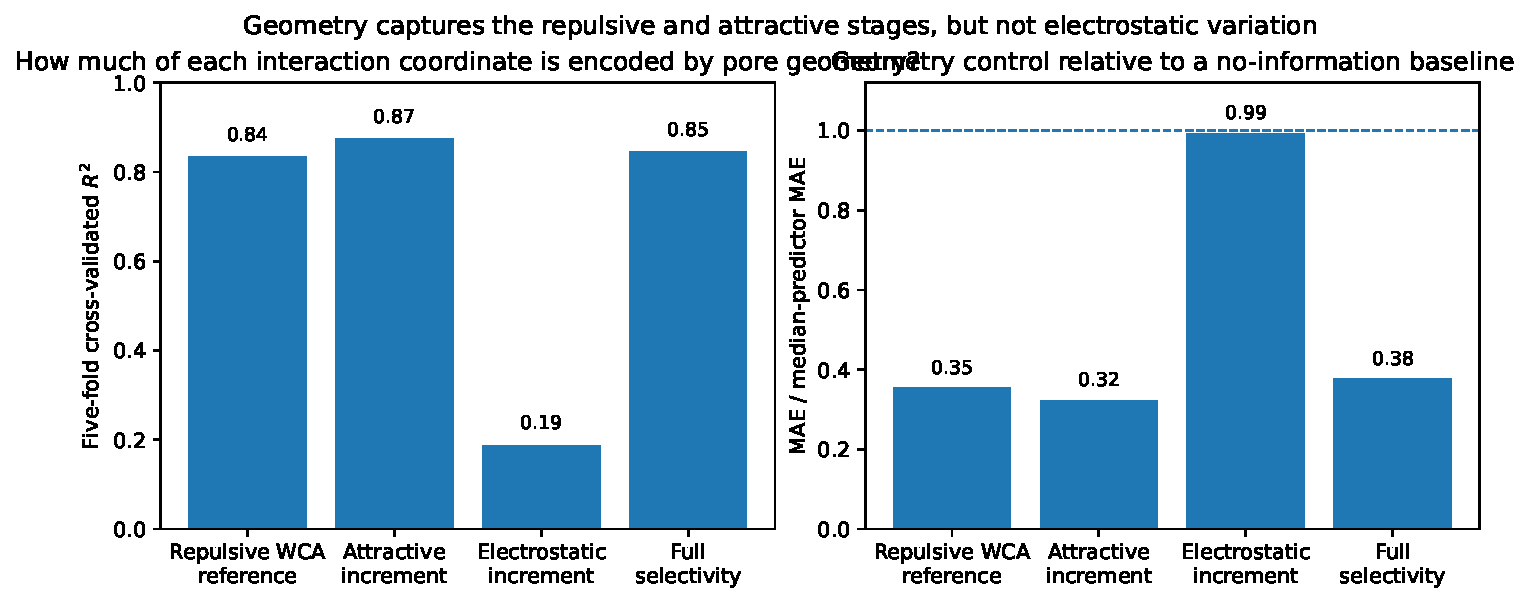
\includegraphics[width=\linewidth]{fig3_geometry_information.pdf}
\caption{\textbf{Geometry predicts the final endpoint while providing little practical gain for the electrostatic increment.} Left: five-fold cross-validated $R^2$ of geometry-only ExtraTrees models. Right: model MAE normalized by the corresponding median-predictor MAE; a value of one indicates no improvement over that baseline.}
\label{fig:geometry}
\end{figure}

\subsection{A geometry-matched pair exposes framework-specific electrostatic recognition}

M029 and M085 form the strongest local counterexample. In the standardized nine-descriptor geometry space used for matched-pair selection, they are mutual nearest neighbors (distance 0.258). Their repulsive log-selectivities are correspondingly close, $-0.201$ and $-0.198$. Yet their electrostatic increments are 0.141 and 2.001, a difference of 1.860, corresponding to a 6.42-fold contrast in the multiplicative electrostatic contribution.

The global Henry coefficients identify which gas drives this divergence. Restoring electrostatics changes $\ln K_H$ for CO$_2$ by 0.162 in M029 and 2.032 in M085, whereas the N$_2$ changes are only 0.021 and 0.032. The between-framework difference is therefore 1.871 log units for CO$_2$ but only 0.011 for N$_2$: the much larger electrostatic selectivity of M085 is overwhelmingly CO$_2$-driven.

Local insertion fields provide a spatial counterpart to this scalar result. Within the 99.5\%-probability-supported pore region, M029 remains close to locally neutral over much of the accessible volume, whereas M085 shows a substantially more positive and heterogeneous full-minus-LJ selectivity response. The probability-weighted median local increment is 0.042 for M029 and 0.534 for M085; 57.6\% and 79.1\% of the corresponding probability weight lies in regions with positive local electrostatic selectivity increments. These maps localize the electrostatic perturbation but do not identify a specific binding motif.

\begin{figure}[H]
\centering
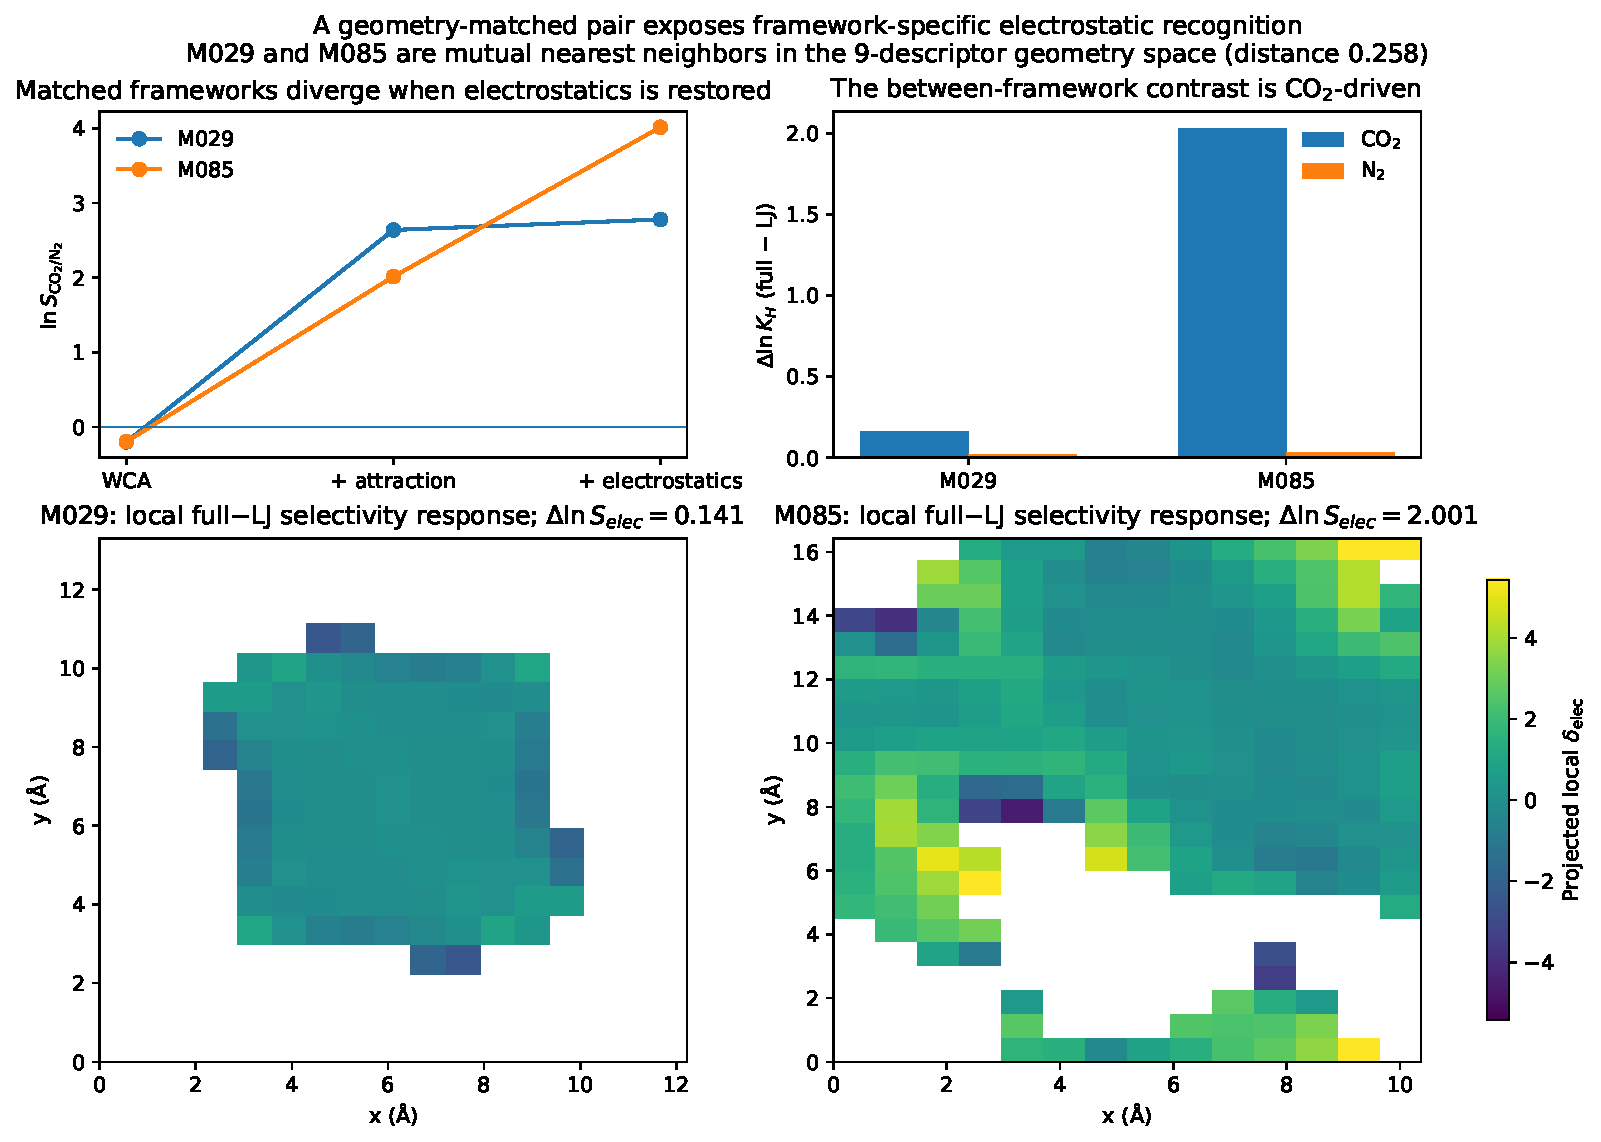
\includegraphics[width=\linewidth]{fig4_matched_electrostatic.pdf}
\caption{\textbf{A geometry-matched pair exposes framework-specific electrostatic recognition.} M029 and M085 are mutual nearest neighbors in the geometry space used for pair selection. Top left: selectivity trajectories through WCA, LJ-only, and full interaction states. Top right: gas-specific global full-minus-LJ changes in $\ln K_H$, showing that the between-framework contrast is dominated by CO$_2$. Bottom: probability-supported local full-minus-LJ selectivity increments. Global increments are taken from the Henry calculations; spatial fields are used only to localize the response.}
\label{fig:matched}
\end{figure}

\subsection{Attraction and electrostatics reorder candidates in different ways}

Restoring attraction changes the candidate ordering globally. The Spearman correlation between WCA and LJ-only ranks is $-0.751$, and the median absolute rank displacement is 102 positions among 238 frameworks. The largest attraction-driven promotion is 234 positions and the largest demotion is 226.

Electrostatics has a different population-level effect. LJ-only and full ranks remain strongly correlated ($\rho=0.905$), with a median absolute displacement of only 9 positions. Nevertheless, specific frameworks are strongly affected: the largest electrostatic promotion is 175 positions and the largest demotion is 55. Attraction therefore reorganizes the ranking broadly, whereas electrostatics mostly preserves the global ordering while creating important framework-specific outliers.

\begin{figure}[H]
\centering
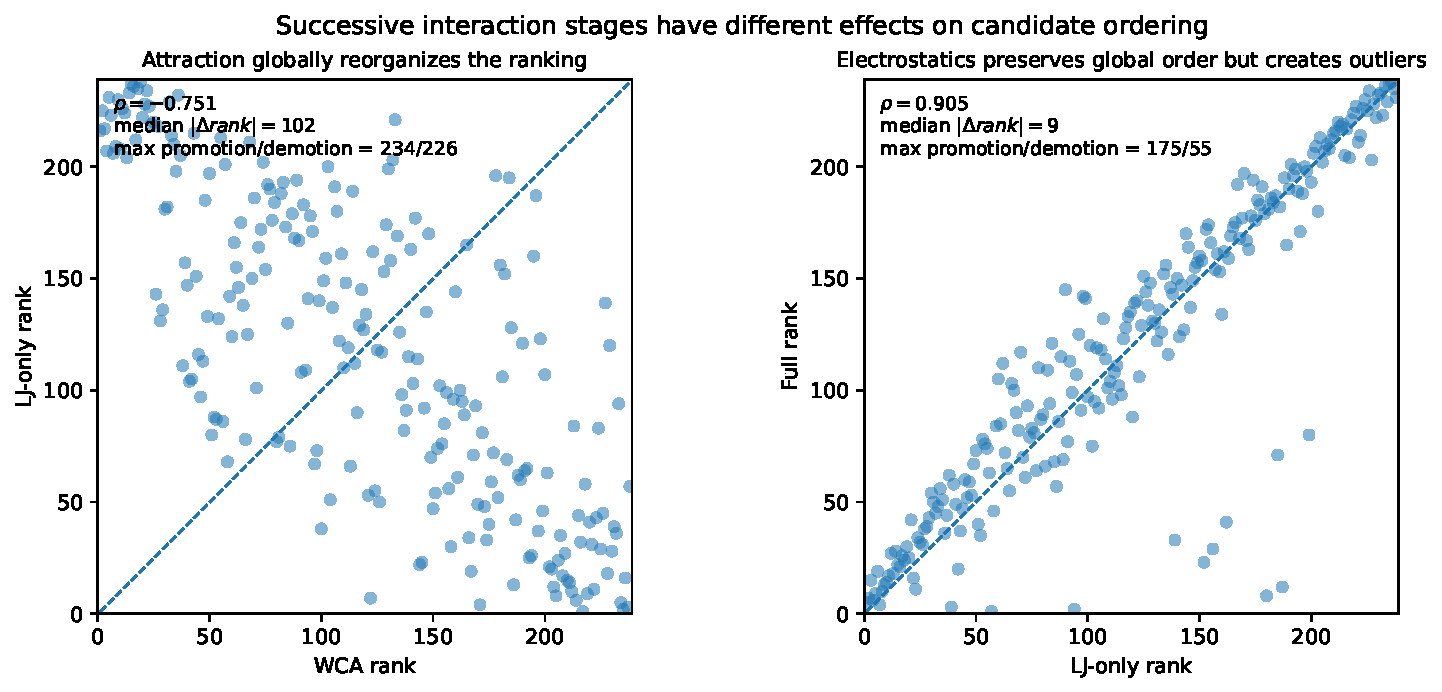
\includegraphics[width=\linewidth]{fig5_rank_trajectories.pdf}
\caption{\textbf{Successive interaction stages have different effects on candidate ordering.} Every point is one MOF. Restoring attraction broadly reorganizes the WCA ranking, whereas restoring electrostatics leaves the global LJ-only ordering much more intact but produces large outlier promotions. Dashed lines denote unchanged rank.}
\label{fig:ranks}
\end{figure}

\section{Discussion}

Previous high-throughput studies established that electrostatics is important for CO$_2$/N$_2$ adsorption and that turning framework charges off can change both Henry selectivities and the identity of top candidates \cite{haldoupis2012charges,daglar2018screening}. The present decomposition refines that conclusion. In this panel, electrostatics is not the interaction stage that first creates CO$_2$ preference: the WCA reference is N$_2$-favoring throughout, and restoring Lennard--Jones attraction alone reverses that baseline throughout. Electrostatics then acts as a second, strongly framework-dependent recognition coordinate.

The representation result provides a complementary distinction. Geometry-based screening has long been useful for low-pressure adsorption \cite{fernandez2016geometry}, while chemistry-aware descriptors improve CO$_2$ working-capacity and selectivity prediction in large MOF libraries \cite{burner2020deeplearning}. Our results locate one reason for that hierarchy. The same conventional pore geometry that predicts $\ln S_{\rm full}$ accurately captures the repulsive and attractive coordinates but barely improves absolute prediction error for $\Delta\ln S_{\rm elec}$. Endpoint accuracy can therefore hide a representation boundary: a model may predict the final number without resolving one of the physical increments that constructs it.

The M029/M085 pair turns that population result into a controlled local comparison. The two structures are mutual nearest neighbors in the geometry space used for pair selection and have almost identical WCA selectivities, yet their electrostatic responses differ by 1.860 log units. The contrast is almost entirely associated with CO$_2$, and the insertion fields show a correspondingly stronger and more heterogeneous local response in M085. The maps do not establish which atom type or chemical motif is responsible; that requires a validated chemistry-aware local representation beyond the scope of the present study.

The ranking analysis shows why retaining the interaction coordinates matters for screening. Attraction changes the ordering of the panel globally, consistent with its role in reversing the repulsive baseline. Electrostatics leaves the overall LJ-only order more recognizable but can still rescue individual frameworks by more than 100 positions. A final rank therefore answers which material performs well under the complete model, whereas the nested coordinates reveal how it became competitive.

The conclusions are deliberately bounded to Henry-regime thermodynamic recognition at 298~K in rigid frameworks under the selected molecular models. A preselected 15-MOF DREIDING-linker/UFF-Co bridge produced only small changes in the WCA excess chemical potentials and essentially unchanged WCA rankings (Supporting Information), supporting the repulsive-baseline interpretation within that perturbation. Equivalent force-field robustness has not been established for the LJ-only or electrostatic increments. The study does not address finite-pressure mixtures, transport, framework flexibility, or transfer to other gas pairs.

\section{Methods}

\subsection{Framework panel and molecular models}

The starting panel contained 240 ARC--MOF structures \cite{burner2023arcmof}; 238 had the complete WCA, LJ-only, and full CO$_2$/N$_2$ quantities required for the common analysis. Frameworks were treated as rigid at 298~K. Full and LJ-only Henry calculations used RASPA3 version 3.0.29 \cite{ran2024raspa3,dubbeldam2016raspa}. The framework Lennard--Jones model used element-level UFF parameters \cite{rappe1992uff} with Lorentz--Berthelot mixing, a 12~\AA{} cutoff, shifted truncation, and no tail correction. Framework charges were taken from the ARC--MOF structure records. Full calculations used Ewald electrostatics; LJ-only calculations set framework and guest pseudoatom charges to zero while preserving the Lennard--Jones definitions.

The full calculation used 50,000 Widom cycles per seed and the LJ-only calculation used 10,000 cycles per seed, with three matched default seeds and adaptive extension of unresolved cases. The exact protocol, guest geometries, and retained RASPA force-field definitions are archived with the publication source data.

\subsection{Nested reference potentials}

For gas $g$ and interaction state $x$, the Henry-regime selectivity is
\begin{equation}
\ln S_x
=
\ln K_{H,\mathrm{CO_2}}^x
-
\ln K_{H,\mathrm{N_2}}^x,
\qquad
x\in\{\mathrm{WCA},\mathrm{LJ},\mathrm{full}\}.
\end{equation}
The two increments are
\begin{align}
\Delta\ln S_{\rm attr} &= \ln S_{\rm LJ}-\ln S_{\rm WCA},\\
\Delta\ln S_{\rm elec} &= \ln S_{\rm full}-\ln S_{\rm LJ}.
\end{align}

For the WCA state, each framework--guest Lennard--Jones pair potential was truncated at
$r_{c,ij}=2^{1/6}\sigma_{ij}$ and shifted to zero at the cutoff. Molecular Widom insertion \cite{widom1963} was used to evaluate the repulsive reference. Independent equal-length WCA seeds were pooled in Boltzmann-factor space before conversion back to the excess chemical potential. Seed counts, precision diagnostics, and exclusion sensitivity are reported in the Supporting Information.

\subsection{Geometry information analysis}

The geometry-only analysis used 14 conventional pre-simulation descriptors. Target-derived adsorption quantities, identifiers, filenames, cluster labels, and other variables that could encode the response were excluded before fitting. ExtraTrees regressors used 500 trees, minimum leaf size three, a maximum-feature fraction of 0.7, and five-fold shuffled cross-validation with random seed 20260918. Prediction was used as an information-content diagnostic rather than as the primary objective. Performance was evaluated with $R^2$, MAE, and the MAE of a median predictor.

\subsection{Matched-pair analysis}

Matched pairs were selected from the closest 2\% of all framework pairs in a standardized nine-descriptor geometry space and then ranked by contrast in the target mechanistic coordinate. The retained attraction pair is M089/M192 and the retained electrostatic pair is M029/M085. For the electrostatic pair, M029 and M085 are mutual nearest neighbors in that geometry space. Pair selection preceded the spatial interpretation.

\subsection{Spatial insertion fields}

Spatial fields were computed on a fixed 0.75~\AA{} grid using the validated fixed-position RASPA/RASPALIB evaluator and the same rigid guest geometries, framework structures, Lennard--Jones parameters, charge assignments, mixing rules, and temperature as the corresponding Henry calculations. At each position $\mathbf r$,
\begin{equation}
w(\mathbf r)=
\left\langle
\exp[-\beta U(\mathbf r,\Omega)]
\right\rangle_{\Omega}.
\end{equation}
LJ-only fields used 2,048 orientations per voxel. Full fields used 16,384 or 32,768 orientations; targeted nested 16k$\rightarrow$32k$\rightarrow$64k checks at probability-important voxels changed the tested values by at most approximately 0.04\%.

For the electrostatic pair,
\begin{equation}
\delta_{\rm elec}(\mathbf r)
=
\left[
\ln w_{\rm full}^{\mathrm{CO_2}}(\mathbf r)
-\ln w_{\rm full}^{\mathrm{N_2}}(\mathbf r)
\right]
-
\left[
\ln w_{\rm LJ}^{\mathrm{CO_2}}(\mathbf r)
-\ln w_{\rm LJ}^{\mathrm{N_2}}(\mathbf r)
\right].
\end{equation}
Visualization and local summaries were restricted to the union of the minimal voxel sets carrying 99.5\% of the insertion probability of the relevant fields. Local quantities were weighted by normalized insertion probability, preventing inaccessible framework-overlap voxels from dominating logarithmic averages. The spatial fields are localization diagnostics; the global Henry calculations remain the estimator for integrated selectivity increments.

\subsection{Robustness analyses}

The principal signs and the weak attractive--electrostatic association were recomputed after excluding the four WCA cases with $\mathrm{SE}(\ln S_{\rm WCA})>0.10$ and after removing the upper 1\% of each response separately. A preselected 15-MOF bridge additionally replaced supported linker/main-group UFF parameters with DREIDING while retaining UFF for cobalt; all other WCA definitions were preserved. This bridge was used only to test sensitivity of the repulsive-accessibility coordinate to that specified linker-side Lennard--Jones perturbation.

\section{Conclusions}

Across the 238-MOF analysis set, repulsive accessibility alone favors N$_2$, Lennard--Jones attraction reverses this baseline toward CO$_2$ throughout the panel, and electrostatics supplies a further framework-dependent enhancement. The attractive and electrostatic increments are only weakly associated.

Conventional pore geometry captures the repulsive and attractive coordinates strongly and predicts the final selectivity well, yet provides essentially no improvement in absolute electrostatic prediction error over a median baseline. The M029/M085 pair shows the consequence directly: two mutual nearest neighbors in geometry space develop a 1.860-unit difference in electrostatic selectivity, driven overwhelmingly by CO$_2$ and accompanied by markedly different local spatial responses.

Total selectivity is therefore a useful endpoint but an incomplete mechanistic descriptor. The nested reference potentials preserve the route by which a framework becomes selective and reveal when an apparently adequate structural representation predicts the endpoint without resolving the underlying interaction coordinate.

\bibliographystyle{unsrt}
\bibliography{references}
\end{document}
